\documentclass[12pt]{article}
\usepackage[margin=0.75in]{geometry}
\geometry{a4paper}
\usepackage[T1]{fontenc} % Support Icelandic Characters
\usepackage[utf8]{inputenc} % Support Icelandic Characters
\usepackage{graphicx} % Support for including images
\usepackage{hyperref} % Support for hyperlinks
\usepackage{tcolorbox}
\usepackage{lmodern}
\usepackage{lscape}
\usepackage{graphicx}

% (2) specify encoding
\usepackage[T1]{fontenc}

% (3) load symbol definitions
\usepackage{textcomp}

%------------------------------------------------------------------
% TITLE
%------------------------------------------------------------------
\title{
\centerline{
\includegraphics[width=75mm]{images/logo.jpg}}
\vspace{0.8 cm}
 \begin{huge}  
 \textbf{Faculty of Computer Science and Business Information Systems}\\  
\end{huge}  
\\Computer Science (Bachelor of Engineering)\\ [0.60in]
Exam Quality Control
\large  \\[0.60in]
5100240, Programming Project, 2023-2 \\ 


\small Technical University of Applied Sciences Würzburg-Schweinfurt - Faculty of Computer Science and Business Information Systems, Sanderheinrichsleitenweg 20
97074 Würzburg.

  }
  


\author{
    KAAN ÖZER\\
    \textbf{Computer Science}\\
    \texttt{9123043}\\[0.20in]
    \and
    Kemal Öztürk \\
    \textbf{Computer Science}\\
    \texttt{5122100}\\[0.20in]
    \and
    Müberra Şeyma USLU \\
    \textbf{Computer Science}\\
    \texttt{9123059}\\[0.20in]
    \and
    Illia Rohalskyi\\
    \textbf{Computer Science}\\
    \texttt{9123047}\\[0.20in]
    \and
}


\date{8. May 2023}\\







%------------------------------------------------------------------
% DOCUMENT STARTS HERE
%------------------------------------------------------------------
\begin{document}
\maketitle

\pagenumbering{roman}
\newpage
\tableofcontents


\newpage
\pagenumbering{arabic} 

\section{Introduction}
\subsection{Context of the Work}
The "Exam Quality Control" program aims to address the challenges faced in managing and evaluating exam schedules in educational institutions and organizations. Creating effective and fair exam schedules while following various rules and constraints can be difficult. Manual evaluation of exam plans is time-consuming and prone to mistakes. Therefore, it is essential to develop an automated software solution that can examine exam schedules based on predefined rules.
\subsection{Motivation for This Work}
The motivation behind developing the "Exam Quality Control" program is to evaluate the current exam schedule with utmost accuracy and efficiency. The main objective is to identify any conflicts between the evaluated exam plan and the specified rules and assist in creating the subsequent exam schedule that adheres as closely as possible to these rules. By automating this process, our institution can simplify their scheduling procedures, reduce conflicts, and improve the overall quality of exams. This software gives administrators and schedulers a reliable tool to follow regulations, allocate resources effectively, and provide the best possible exam experience for both students and examiners.
\subsection{Objective for This Work}
The primary objective of the "Exam Quality Control" program is to provide a comprehensive and automated solution for evaluating exam schedules based on predefined rules. The software will consider multiple rules during the evaluation process, including:\vspace{\baselineskip}

    \textbf{Big Exams Early:} \vspace{\baselineskip}
    Big exams should be held early.
    
    \textbf{One Day Gap:} \vspace{\baselineskip}
    There should be one day gap between each two exams.
    
    \textbf{One Exam Per Day:} \vspace{\baselineskip}
    There should be only one exam per day for each student.
    
    \textbf{Special Dates:} \vspace{\baselineskip}
    Examiners shouldn't come in specific dates.
    
    \textbf{Special Professors:} \vspace{\baselineskip}
    The distance between the two exam shouldn't be so long if the examiner is same. Additionally, the number of exams that assigned to the examiners should be in a balance.
    
    
    \textbf{Room Capacity:}\vspace{\baselineskip}
    The number of students and the capacity of the rooms should be in a balance.
    
    \textbf{Room Distances:} 
    If one exam is conducted in more than one room, the distance between them should be minimal.

         
 
\vspace{\baselineskip}
    

By evaluating exam schedules based on these rules and potentially additional ones, the software will provide scores for each rule, enabling administrators to identify areas for improvement and make data-driven decisions to optimize the overall exam plan. The objective is to simplify the scheduling process, enhance the quality of exam plans, and improve the overall experience for both students and examiners.

\vspace{\baselineskip}

\section{Technical Foundations}

\subsection{Regression basics:}

 In the context of this work, \textit{linear regression} is a technique that aims to find a line that best fits a given set of data points. It does so by minimizing the distance between the line and the data points. The formula of the line is $y = mx + b$, which represents a straight line.

\textit{Polynomial regression} refers to a line that has $N$ number of polynomials in its formula. The formula for polynomial regression is given by $y = M_{n}X^{n} + M_{n-1}X^{n-1} + \ldots + m_{1}x + b$, where $m$ is the slope and $b$ is the intercept. Both the parameters $m$ and $b$ are approximated by regression. The degree $N$ of the polynomial is determined heuristically. Using polynomials enables the line to be non-linear and have some curvature.

\section{Evaluation of Project Results}
\subsection{Description of the current status:}

The application is currently in an operational state, allowing users to input their exam plans for evaluation. The system utilizes algorithms and rule-based systems to process the exam plans based on the predefined criteria. It assigns weights to each criterion to reflect their importance in the overall assessment.


\vspace{\baselineskip}


The rules are as follows:

\begin{itemize}
\item Big exams have to be early.
\item Students mustn't have two exams on the same day.
\item Students should have one day gap between exams.
\item Rooms have to be neither too big nor too small for the exam.
\item If two rooms are assigned for the exam, they have to be as close as possible.
\item The professor is not available on some dates.
\item The professor wants to come on a minimal amount of days.
\end{itemize}

The current version of the application provides a score indicating the overall quality of the exam plan. Additionally, it generates an HTML report file that includes visualizations, conflict dataframes, and scores for each individual criterion. This report serves as a valuable tool to help professors spot potential problems and gain insights into the strengths and weaknesses of the exam plan.

\subsection{Functional requirements:}


The application should assess the exam plans based on predefined criteria, evaluating each criterion individually. The perfect exam plan would satisfy both, professors and students. Thus, we should aim to provide a comprehensive solution that would take into consideration both perspectives.

\vspace{\baselineskip}


The application should calculate an overall score for each exam plan, indicating its quality. The scoring mechanism will be based on weighted averages, taking into account the relative importance of each criterion.

\vspace{\baselineskip}


The application should provide detailed explanations for the assigned score, clearly stating the reasoning and factors that contributed to it. This feature helps professors understand the strengths and weaknesses of the exam plan and provides transparency in the evaluation process.

\vspace{\baselineskip}


The application should generate an HTML report file, presenting visualizations, conflict dataframes, and scores for each individual criterion. The report should be easily accessible and designed in a clear and intuitive manner, allowing professors to review the assessment results effectively.

\vspace{\baselineskip}


The application should have conflict detection capabilities, identifying any conflicts within the exam plan. It should highlight inconsistencies or contradictions between criteria in the report, enabling professors to address and resolve these conflicts during the exam planning process.

\vspace{\baselineskip}


By fulfilling these functional requirements, the solution aims to comprehensively evaluate exam plans, calculate scores, provide explainability, generate informative HTML reports, and assist professors in identifying and resolving conflicts to enhance the quality of their assessments.


\subsection{Non-functional requirements:}


The application should be reliable, ensuring accurate and consistent evaluation results. It should be able to handle errors and exceptions gracefully, with minimal impact on the overall functionality. On top of that, the application should be designed and developed with maintainability in mind, allowing for easy updates, bug fixes, and future enhancements



\section{Description of the Solution}
\subsection{Description of the software architecture}



Our software consists of three layers which are Input, Process, and Output layers. Data layer.

\vspace{\baselineskip}

The input layer is responsible for the preprocessing of examination plan files, enabling their utilization within the software.

\vspace{\baselineskip}

The process layer is responsible for analyzing the exam plan data to score, identifying conflicts, and visualizing data based on rules such as ensuring a one-day gap between exams.


\vspace{\baselineskip}

The output data is responsible for representing the scores, conflicts, and charts of every rule in a HTML file.

\FloatBarrier
\begin{figure}[ht]
    \centering
    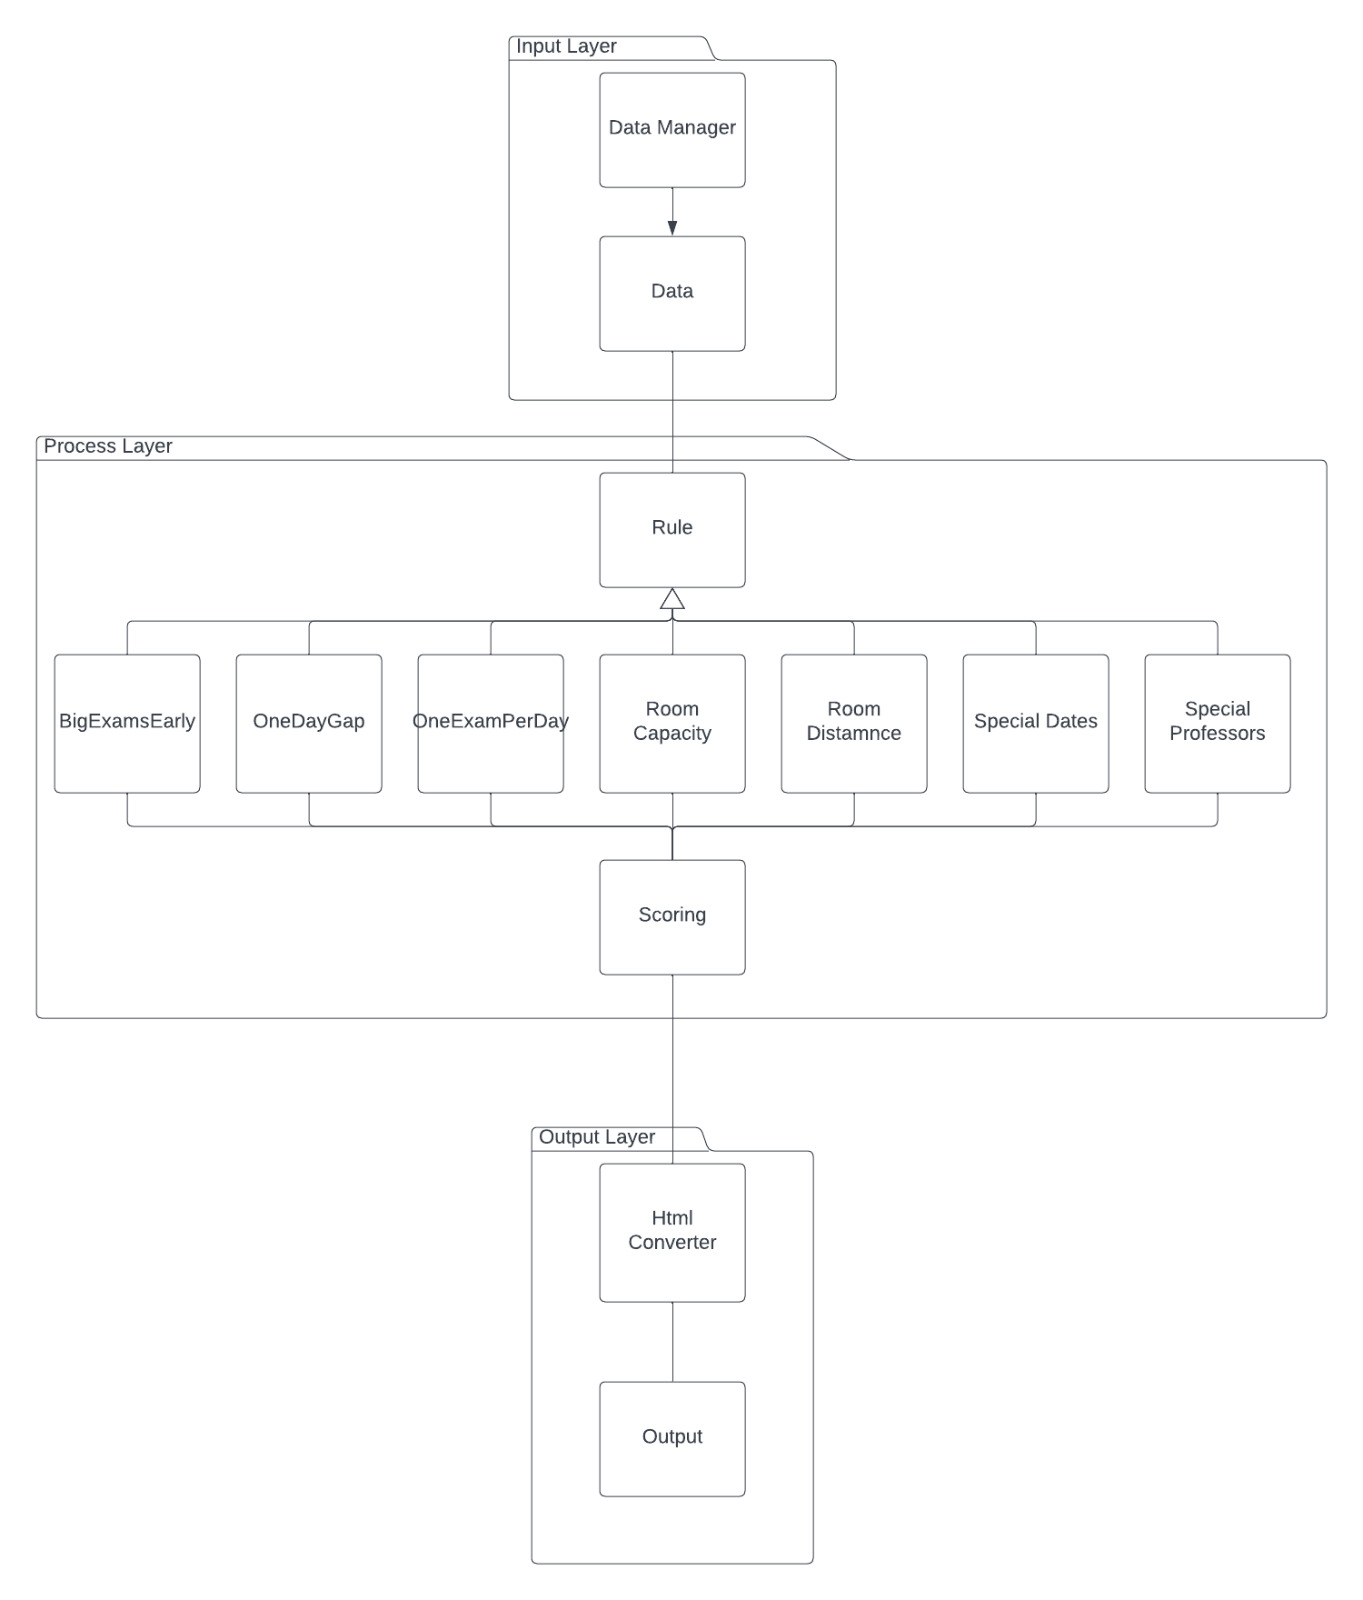
\includegraphics[width=160mm]{images/architecture.jpg}
    \caption{Architecture Design}
    \label{fig:entrance-screen}
\end{figure}
\FloatBarrier



\subsection{Overview and interaction of the components}

\subsubsection{Main Class}


\begin{itemize}
\item This class is responsible from the execution of the program and saving the various html results based on the demand.
\end{itemize}




\subsubsection{Scoring Class}


\begin{itemize}
\item Scoring class interacts with the following rule classes: BigExamsEarly, OneExamPerDay, RoomCapacity, RoomDistance, SpecialProfessors, OneDayGap, SpecialDates.
\item This class is a wrapper for all of the rule classes. It is made to make it easy to access each of the components under one class.
\end{itemize}


\subsubsection{Data Class}


\begin{itemize}
\item The Data class is responsible for importing and organizing the input data from various files.
\item It can load different types of data such as CSV, JSON, and Excel. The following are the files that the Data class interacts with: \texttt{FIW\_Exams\_2022ws.xlsx}, \texttt{Pruefungsanmeldungen\_anonmous.csv}, \texttt{room\_distance\_matrix.xlsx}, \texttt{capacity.json}, \texttt{special\_dates.csv}, \texttt{specific\_professors.xlsx}.
\item It also splits and extracts relevant information from the loaded data and stores them as attributes and methods for further processing.
\item All of the rule classes interact with Data. It is a prerequisite for them to work.
\end{itemize}


\subsubsection{Rule Class}

Rule is the superclass of all scoring classes (such as BigExamsEarly, OneExamPerDay, etc.).

\vspace{\baselineskip}

The class has the following attributes:

\begin{itemize}
\item score.
\item conflicts.
\item plot array.
\end{itemize}
 
It has a method called compute() which returns the score, conflicts, and plot array.

\subsubsection{Data Manager Class}

DataManager is a class to instantiate Data objects. The class provides methods to create and retrieve instances of the Data class. It ensures that only a single instance of the Data class is created and reused throughout the program.

\vspace{\baselineskip}

\subsubsection{BigExamsEarly Class}


\begin{itemize}
\item Big exams should be held early in the exam period, and this class calculates the score and evaluates the exam plan based on the number of big exams and their scheduling time.
\end{itemize}


\subsubsection{OneExamPerDay Class}


\begin{itemize}
\item Verifies whether each student has only one exam scheduled per day.
\item Gives a penalty score while calculating the score of the exam plan based on the number of students who has multiple exams in a day.
\end{itemize}

\subsubsection{OneDayGap Class}


\begin{itemize}
\item This class calculates the score based on the absence of a one-day gap between exams for the same student.
\item basically identifies cases where there is no one-day gap between exams for the same student and calculates a general score for this rule by giving penalty based on the number of conflicts and also draws a plot showing the relationship between the number of conflicts and the score.
\end{itemize}

\subsubsection{RoomCapacity Class}


\begin{itemize}
\item Ensures that the assigned rooms can accommodate the number of students registered for each exam.
\item Computes the score by comparing the number of students with the room capacities for the each exam.
\end{itemize}

\subsubsection{RoomDistance Class}


\begin{itemize}
\item It search the rooms for each exam and if there is more than one room. It calculates the sub-scores of the distance between the relevant rooms.
\item This class has only score as its output.
\end{itemize}

\subsubsection{SpecialDates Class}


\begin{itemize}
\item This class is responsible for calculating the score for examiners, which are not able to come for the exam on a specific day.
\item Checks for conflicts between examiners' names and special dates in the \verb|special_dates_df|.
\item Import data class to reach \verb|special_dates_df| .
\item if there is a match, it adds the conflict information to the 'conflicts' list and makes a binary decision.
\item It returns a percentage score based on whether there is a conflict or not.
\end{itemize}

\subsubsection{SpecialProfessors Class}


\begin{itemize}
\item This class calculates special professors score based on the number of exams and the distance between those exam days that same professors supervise.

\end{itemize}






\subsubsection{Output Class}


\begin{itemize}
\item Handles the generation and saving of output files.
\item Provides methods for saving the results as HTML files. These methods offers two different option either you can get a single result of one rule class or a summary list that includes all results.
\item Utilizes the HtmlConverter class to convert data into HTML format and print the output.
\end{itemize}


\subsubsection{HtmlConverter Class}


\begin{itemize}
\item Converts the processed data into HTML format for output representation.
\item Provides methods for creating HTML pages, and printing the HTML output.

\end{itemize}




 \subsection{Quality Assurance}
 
 \subsubsection{Introduction}

 This document presents the Quality Assurance strategy that has been employed for the evaluation
of our existing examination scheduling system. We utilized Python's unittest framework to
construct and perform unit tests for each rule class in the system.


\vspace{\baselineskip}

Each rule class is thoroughly tested under both the best-case and worst-case scenarios. These
scenarios are represented using a combination of mock data, created within the Test methods for
each test case, and artificial data derived from external files. The objective is to mimic a variety of
real-world scenarios.


\vspace{\baselineskip}

These test cases are organized within a dedicated Test class, containing distinct test methods for
each case. For instance, the test methods \texttt{'test\_big\_exams\_early\_best'},  and  \\ 
\texttt{'test\_big\_exams\_early\_worst'} correspond to the best and worst scenarios of the 'big exams early'
rule respectively.



\vspace{\baselineskip}

Our goal with Quality Assurance is to thoroughly test the exam schedule evaluation system under
different scenarios. This helps to make sure our system is strong, trustworthy, and can accurately
check the quality of any exam schedule. We aim to highlight both what's working well and what
could be better in the schedule.

\subsubsection{Module: OneExamPerDay}

 
\vspace{\baselineskip}

 
\textbf{Test1: One Exam Per Day - Best Scenario}


\vspace{\baselineskip}

 
 \textbf{Test Description:}
This tests uses a dataset where students take a maximum of one exam
per day. It tests the rule under optimal conditions and expects a high score.

\vspace{\baselineskip}

\textbf{Input:}
 Mock data where all students in exam plan take maximum one exam per day.


\vspace{\baselineskip}

\textbf{Expected Result:}
Score is approximately 100 out of 100. This indicates that the scheduling
system is functioning properly for the best-case scenario.



\vspace{\baselineskip}


 
\textbf{Test2: One Exam Per Day - Worst Scenario}


\vspace{\baselineskip}

 
 \textbf{Test Description:}
This tests uses a dataset where students take more than one exam per
day. It tests the rule under optimal conditions and expects a low score.

\vspace{\baselineskip}

\textbf{Input:}
Mock data where all students in exam plan take more than one exam per day.


\vspace{\baselineskip}

 
 \textbf{Expected Result:}
Score is approximately 0 out of 100. This indicates that the scheduling
system is functioning properly for the worst-case scenario.


\vspace{\baselineskip}

\subsubsection{Module: SpecialDates}

 
\vspace{\baselineskip}

 
\textbf{Test1: Special Dates - Best scenario}


\vspace{\baselineskip}

 
 \textbf{Test Description:}
This test uses a dataset where examiners don’t have to supervise exams
in his/her special specific dates.


\vspace{\baselineskip}

\textbf{Input:}
Mock data where all examiners don’t supervise exams in specific dates.



\vspace{\baselineskip}

\textbf{Expected Result:}
Score is approximately 100 out of 100. This indicates that the scheduling
system is functioning properly for the best-case scenario.


\vspace{\baselineskip}


 
\textbf{Test2: Special Dates - Worst scenario}


\vspace{\baselineskip}

 
 \textbf{Test Description:}
 This test uses a dataset where examiners have to supervise exams in
his/her special specific dates.


\vspace{\baselineskip}

\textbf{Input:}
Mock data where all examiners supervise exams in specific dates.


\vspace{\baselineskip}

 
 \textbf{Expected Result:}
 Score is approximately 0 out of 100. This indicates that the scheduling
system is functioning properly for the worst-case scenario.


\vspace{\baselineskip}



 \subsubsection{Module: BigExamsEarly}

 
\vspace{\baselineskip}

 
 \textbf{Test 1: Big Exams Early - Best Scenario}


\vspace{\baselineskip}

 
 \textbf{Test Description:}
 This test uses a dataset where the bigger exams are scheduled early. It tests
the rule under optimal conditions and expects a high score.


\vspace{\baselineskip}


 \textbf{Input:}
 Mock data where larger exams are scheduled earlier in the exam schedule.


\vspace{\baselineskip}

 
 \textbf{Expected Result:}
 Score is greater or equal to 70. This indicates that the scheduling system is
functioning properly for the best-case scenario and bigger exams are indeed scheduled earlier.


\vspace{\baselineskip}

 
 \textbf{Test 2: Big Exams Early - Worst Scenario}


\vspace{\baselineskip}

 
 \textbf{Test Description:}
This test uses a dataset where the bigger exams are scheduled late. It tests the
rule under the worst conditions and expects a low score.


\vspace{\baselineskip}


 \textbf{Input:}
 Mock data where larger exams are scheduled later in the exam schedule.


\vspace{\baselineskip}

 
 \textbf{Expected Result:}
 Score is less or equal to 5. This indicates that the scheduling system properly
penalizes scenarios where bigger exams occur late in the schedule.


\vspace{\baselineskip}



 \subsubsection{Module: RoomDistance}

 
\vspace{\baselineskip}


 
 \textbf{Test 1: Room Distance - Best Scenario}


\vspace{\baselineskip}

 
 \textbf{Test Description:}
 This test uses a dataset where students are allocated in rooms close to each
other. It tests the rule under optimal conditions and expects a high score.


\vspace{\baselineskip}


 \textbf{Input:}
A combination of mock data that is either directly created as a dataframe or drawn from
artificial datasets like Excel files. Both types of data are later assigned to the attributes of the
Mock class. This dataset simulates a situation where students' allocated exam rooms are in close
proximity, thus representing an optimal scenario for the room distance rule.

\vspace{\baselineskip}

 
 \textbf{Expected Result:}
 Score is approximately equal to 100. This indicates that the scheduling system
is functioning properly for the best-case scenario and the exams are scheduled in rooms close to
each other.


\vspace{\baselineskip}

 
 \textbf{Test 2: Room Distance - Worst Scenario}


\vspace{\baselineskip}

 
 \textbf{Test Description:}
This test uses a dataset where students are allocated in rooms far from each
other. It tests the rule under the worst conditions and expects a low score.


\vspace{\baselineskip}


 \textbf{Input:}
 A combination of mock data that is either directly created as a dataframe or drawn from
artificial datasets like Excel files. Both types of data are later assigned to the attributes of the
Mock class. This dataset simulates a situation where students' allocated exam rooms are far
apart, thus representing the worst-case scenario for the room distance rule.


\vspace{\baselineskip}

 
 \textbf{Expected Result:}
Score is approximately equal to 0. This indicates that the scheduling system
properly penalizes scenarios where exams are scheduled in rooms far from each other.


\vspace{\baselineskip}



 \subsubsection{Module: OneDayGap}

 
\vspace{\baselineskip}


 
 \textbf{Test 1: One Day Gap - Best Scenario}


\vspace{\baselineskip}

 
 \textbf{Test Description:}
 This test uses a dataset where students have at least one day gap between
their exams. It tests the rule under optimal conditions and expects a score close to 100, indicating
no conflicts.
\vspace{\baselineskip}


 \textbf{Input:}
Mock data (coming from artificial datasets like Excel files, which are passed to the Data
class as parameters), where all students have at least one day gap between their exams.

\vspace{\baselineskip}

 
 \textbf{Expected Result:}
Score is approximately equal to 0, indicating there are no back-to-back exams
for students, which is the ideal scenario.


\vspace{\baselineskip}

 
 \textbf{Test 2: One Day Gap - Worst Scenario}


\vspace{\baselineskip}

 
 \textbf{Test Description:}
This test uses a dataset where students do not have a one day gap between
their exams. It tests the rule under the worst conditions and expects a score close to 0, indicating
high conflicts.

\vspace{\baselineskip}


 \textbf{Input:}
 Mock data where students have exams without a day gap.
 
\vspace{\baselineskip}

 
 \textbf{Expected Result:}
Score is approximately equal to 0. The score is expected to be low, indicating
that the system correctly identifies the situation where students have exams without a one day
gap as a problematic scheduling scenario.


\vspace{\baselineskip}




 \subsubsection{Module: SpecialProfessors}

 
\vspace{\baselineskip}


 
 \textbf{Test 1: Special Professors - Best Scenario}


\vspace{\baselineskip}

 
 \textbf{Test Description:}
This test uses a dataset where special professors have all their exams
scheduled on the same day. It tests the rule under optimal conditions and expects a score close
to 100, indicating no conflicts.

\vspace{\baselineskip}


 \textbf{Input:}
Mock data where all special professors are assigned to multiple examinations on the same
day (for each professor individually), rather than having their exams spread out over separate
days.

\vspace{\baselineskip}

 
 \textbf{Expected Result:}
Score is approximately equal to 100, indicating that all special professors'
exams are scheduled on the same day. This means they aren't required to come to campus on
multiple, separate days, which is the ideal scenario.


\vspace{\baselineskip}

 
 \textbf{Test 2: Special Professors - Worst Scenario}


\vspace{\baselineskip}

 
 \textbf{Test Description:}
This test uses a dataset where special professors are assigned to supervise
examinations on different days, implying they have to be present on campus on multiple separate
days. This is considered the worst-case scenario for this rule and expects a score close to 0,
indicating a large number of conflicts.

\vspace{\baselineskip}


 \textbf{Input:}
Mock data where special professors are assigned to supervise different examinations, each
on a separate day. This is achieved by intentionally designing the mock data such that each
special professor supervises one examination per day, but the exams are scheduled on different
days.
 
\vspace{\baselineskip}

 
 \textbf{Expected Result:}
Score is approximately equal to 0, indicating that special professors' exams are
distributed over several days. This is the least ideal scenario, as it means these special professors
have to come to campus on multiple, separate days, creating a high level of inconvenience.

\vspace{\baselineskip}




 \subsubsection{Module: RoomCapacity}

 
\vspace{\baselineskip}


 
 \textbf{Test 1: Room Capacity - Best Scenario}


\vspace{\baselineskip}

 
 \textbf{Test Description:}
This test uses mock data where the number of students and the capacity of
exam rooms are nearly identical. It tests the room capacity rule under optimal conditions and
expects a high score, indicating the rooms' capacity is efficiently utilized.

\vspace{\baselineskip}


 \textbf{Input:}
Mock data, directly created within the test function, representing a scenario where the
number of students in each course nearly matches the capacity of the assigned exam rooms.

\vspace{\baselineskip}

 
 \textbf{Expected Result:}
Score is greater than or equal to 80, which indicates that room capacities are
efficiently used and there is a balance between the number of students and room capacities. This
implies a proper utilization of resources and an optimal exam scheduling.

\vspace{\baselineskip}

 
 \textbf{Test 2: Room Capacity - Worst Scenario}


\vspace{\baselineskip}

 
 \textbf{Test Description:}
This test uses mock data where the number of students is significantly lower
than the capacity of the assigned exam rooms. It tests the room capacity rule under worst-case
conditions and expects a low score, indicating inefficient usage of room capacities.

\vspace{\baselineskip}


 \textbf{Input:}
Mock data, directly created within the test function, representing a scenario where the
number of students for each course is significantly lower than the capacity of the assigned exam
rooms.
 
\vspace{\baselineskip}

 
 \textbf{Expected Result:}
Score is less than or equal to 10, indicating that the room capacities are not
efficiently used and there is a significant imbalance between the number of students and room
capacities. This implies an inefficient utilization of resources and sub-optimal exam scheduling.

\vspace{\baselineskip}

\subsubsection{Test Results Interpretation}


If all the tests pass, it indicates that the scoring system for the module is working as
expected under both the best and worst scenarios.

\vspace{\baselineskip}


• If any of the tests fail, it suggests a problem with the scoring system in handling that specific
scenario. The console output and failure messages should provide insight into what went
wrong in these cases. The problem may stem from how the score is calculated or how the
input data is processed.
\section{Setup and Operation of the Software Solution}
\subsection{Dependencies on other software system}

The application has dependencies on specific software systems and packages to ensure its smooth functioning. In order for the application to run successfully, Python 3.10.9 must be installed, along with the following required packages:

\begin{itemize}
\item Matplotlib 3.7.0: for data visualization.
\item Pandas 1.5.3: for data manipulation.
\item Numpy 1.23.5: to operate with matrices.
\item Json (comes prebuilt with python): to read json file.
\item Csv (comes prebuilt with python): to read csv file.
\item Byte64 (comes prebuilt with python): required for html creation.
\item Io (comes prebuilt with python): required for html creation.
\end{itemize}




\subsection{Software Availability}

The application is available in a \href{https://bitbucket.student.fiw.fhws.de:8443/projects/PRGPROJSS23/repos/programmierprojekt-ss-23---gruppe-99---exam-quality-control/browse}{BitBucket repository.}  

\vspace{\baselineskip}

The BitBucket repository contains the source code, documentation, and any other relevant resources for the software. By accessing the repository, users can review the code, download the necessary files, or contribute to the development process.

\subsection{Installing the Software:}

To install the software, follow these steps:

\begin{itemize}
\item Access the BitBucket repository using the provided link.
\item Clone the repository to your local machine by either downloading the repository as a ZIP file or using a Git client to clone the repository.
\item Ensure that Python 3.10.9 is installed on your system. If not, download and install Python 3.10.9 from the official \href{https://www.python.org}{Python website .} 
\item Open a command-line interface or terminal and navigate to the location where the repository was cloned or extracted.
\end{itemize}






Install the required dependencies (Matplotlib, NumPy, Pandas) by executing the following command:


\begin{itemize}
 
\item pip install -r requirements.txt
\end{itemize}

This command will install all the required packages specified in the requirements.txt file.
Once the dependencies are installed, the software is ready to run.


\subsection{Opportunities for later adaptation and further development}
There are several potential areas for future development and improvement of the application. Let's discuss the suggested enhancements:

\vspace{\baselineskip}

One could improve scoring system by including information about which examiners failed the exam and have to retake it. It can be a valuable addition to the scoring system. By considering individual examiner failures, the system can provide a fairer evaluation of exam plans, penalizing them less for consecutive exams for those specific students. This enhancement would require modifying the evaluation criteria and calculation algorithms to incorporate examiner failure data. By the time we were developing the project, we did not have data for that.

\vspace{\baselineskip}

To enhance the user experience and make the application more user-friendly, improvements can be made to the installation process. This could involve creating an installer or package that simplifies the installation steps, automatically handles dependencies, and provides clear instructions for setting up and running the application. Additionally, providing a user-friendly installation guide or script can help streamline the installation process.

\vspace{\baselineskip}

Also developing a Graphical User Interface (GUI) for the application can significantly enhance the user experience. A GUI would provide a visual interface with intuitive controls and interactive elements, making it easier for professors to input exam plans, view evaluation results, and interact with the system. The GUI can incorporate features such as drag-and-drop functionality, visual representations of data, and real-time updates, offering a more engaging and efficient user experience.
\section{Retrospective}
\subsection{Evaluation of the project results}

The team's assessment of the project is that while it is not considered fully complete, it showcases promising potential for further enhancements, as mentioned earlier. However, the inner logic of the application is well-designed and demonstrates a high level of quality. The project successfully incorporates multiple evaluation criteria and effectively models them in an efficient and robust manner. This accomplishment represents a significant step forward in providing a viable solution to the problem of exam scoring.

\vspace{\baselineskip}

The successful implementation of the evaluation criteria demonstrates the team's ability to handle complex requirements and deliver a functional solution. The application's capacity to assess exam plans based on predefined criteria contributes to improving the quality and fairness of the evaluation process. The team's effort in designing and implementing the inner logic of the application is commendable.

\vspace{\baselineskip}


Moving forward, the team acknowledges the areas for improvement highlighted earlier, such as enhancing the scoring system, improving installability, and developing a graphical user interface. By addressing these aspects, the application can be further refined to offer an even better user experience and provide more accurate evaluation results.


\vspace{\baselineskip}


Overall, the team's evaluation of the project is positive, recognizing the solid foundation and potential for future improvements. The successful implementation of the inner logic and the incorporation of multiple evaluation criteria demonstrate the team's competence and commitment to delivering a valuable solution to the problem of exam scoring.

\subsection{Project management method and tools used}

The project team employed the Agile and Scrum methodologies for project management. These methodologies provided a suitable framework for managing the workload while maintaining flexibility in terms of work schedules. Here are some details regarding the project management method and tools used:

\vspace{\baselineskip}

For our project, we used Agile and Scrum methodologies. Agile principles emphasize flexibility, collaboration, and iterative development. Scrum, a specific Agile framework, was adopted to organize the work into time-boxed iterations (sprints) and facilitate regular communication and feedback.

\vspace{\baselineskip}

The team members worked individually or in pairs, depending on the task requirements. This approach allowed for a balanced distribution of workload and encouraged collaboration and knowledge sharing among team members.


\vspace{\baselineskip}

The team held regular meetings to ensure effective communication and progress tracking. This included weekly meetings with the supervisor to receive guidance, feedback, and align project goals. Additionally, weekly team meetings were conducted to discuss implementation details, and address any challenges or concerns.

\vspace{\baselineskip}

For the collaboration, we were having a WhatsApp group chat. Maybe it was unprofessional from us, but that made it very easy to collaborate and discuss our project. By doing it in a regular messenger, we established efficient and quick way to communicate. For the version control system, we used BitBucket, which was offered to us in the very beginning of the project.
\subsection{Summary and Outlook}

The technical results of the project are significant, as the team successfully implemented the core functionality of the application. The application provides a scoring system for evaluating exam plans based on predefined criteria, generating reports, visualizations, and identifying conflicts. The implemented solution demonstrates a good understanding of the problem domain and effectively addresses the primary objectives. 


\vspace{\baselineskip}


For the future development, one could refer to part 5.4, where it is broken down in details. But in nutshell: UI, better installability, more rules
Throughout the project process, regular meetings were conducted with the project supervisor and team members to discuss progress, resolve challenges, and align goals. The Agile and Scrum principles guided the iterative development, allowing for flexibility and adapting to changing requirements as needed.




\vspace{\baselineskip}


By following this iterative approach and incorporating stakeholder feedback, the project evolved over time, resulting in an application that addressed the core objectives of scoring exam plans while accommodating potential future enhancements and improvements.





\end{document}

